In this section we will use our tool on a real world use case. % ref stride
% Ref stride, quickly what it is, why our tool, what's the results ?
\subsection{Problem statement}
We want to use symbolic regression on the output of a simulator. The parameter space of the simulator is huge, and a single simulation instance is computationally expensive. We would like to obtain symbolic expressions relating parameters values to simulator output. These expressions can be used to gain insight into which parameters are correlated, which have a larger effect on output and which are irrelevant. 
Given the huge parameter space of the simulator a Design Of Experiment is constructed where the coverage of the parameter space is maximized while minimizing the number of combinations for all parameters. % rewrite this when I have some caffeine in my blood
We then execute the simulator on each configuration. With the execution of a single configuraton independent of all others this is an embarrassingly parallel problem. We combine the output of all configurations and feed them into a tool where we can apply symbolic regression or another machine learning technique in order to extract a model that approximates the simulator. The problem with this approach is twofold. We have to wait until the simulator has completed all configurations and the SR tool executes on a large dataset. It has no known starting point so effectively performs a blind search in a huge search space. We can avoid both issues by using partial results from the simulator as input for the SR tool. The results from these partial samples ideally will provide a good starting point for the incrementally growing dataset. The last assumption only holds if the sequence of completed configurations is a good sample of the full dataset. We can enforce this sequence by ordering the configurations but this is non trivial. Configurations will not have the same computational load for all simulations. Consider for example the population parameter in a epidemiological simulator. An increase in runtime is expected if we increase this parameter. Even if we take this into account in our scheduling, the parallel execution of any number of tasks is never deterministic. The order of configurations is not only important to avoid a bias for the full design, which would lead to overfitting. The initialization problem \ref{subsubinvalidexpressions} reappears here. If the initial partial set of configurations is biased the probability is quite high that the resulting solutions are invalid for the complete data set. 
\subsection{Design of Experiment}
% List DOE technique used and parameter configuration
% Why this technique
\subsubsection{Experiment configuration}
We construct a DOE with 3 parameters, 30 points in total. 
\begin{itemize}
\item initial depth 3
\item maximum depth 6
\item p: population 20
\item g: generations per phase 60
\item f: phases 30
\item archive 4 best per phase
\item d: datapoints : 10, 20, 30
\end{itemize}
The total cost in fitness evaluations is then given by: 20*60*30*d.
We compare 3 approaches. First we run the CSRM tool on the entire dataset. This is the classical approach, the tool is not seeded and so starts a blind search. In a real world setting this would mean waiting until the simulator has run all 30 configurations.
In our second approach we split the data into incremental sections. After 10 configurations have completed we start the tool on this dataset. 
The best 4 results are saved to disk, then we run the tool with the result of 20 configurations and use the results from the previous run as a seed. The overlap between the two datasets will mitigate the initialization problem. Finally we use the results of the 20-point dataset as seed for the 30 point run. 
The cost of running the 10 and 20 point runs to use as seed for the 30 point run is equal to the cost of the 30 point run. 
To ground the comparision our last approach runs the tool on the data from 30 configurations with double the amount of phases. This means that it has the same number of fitness evaluations as the 10-20-30 combination. We compare all three to see which gains are made and at what cost.
\subsection{Results}
\subsubsection{Fitness improvement}
In Figure \ref{fig:incrementalgain} we see that the fitness is improved by using the best results of the previous run on a partial data set. We have deliberately split our data set to expose a risk here. If we run the tool with 20 datapoints seeded by a run of 10 datapoints, we see that the validated fitness actually decreases compared to a non seeded run. The ratio between new and known data is too large, leading to overfitting. If we seed the best results from the 20-point run into a 30 point configuration we see that both the training and validated fitness values significantly improve. 
The 30 point run with 60 phases has the same computational cost as the 10-20-30 runs combined, but has lower convergence. We see that convergence is slowing, with training fitness improving by a factor of 1.1, but validation fitness worsens. This is a typical example of overfitting. The combined 10-20-30 run increases validation fitness with a factor of 1.13. Note the clustering patterns in the incremental runs. When seeded with solutions of previous runs we introduce information that the algorithm otherwise would have to discover. These seeds have fitness values somewhere between the randomly generated and optimal samples. Applying operators on them leads to a niching effect visualized in the fitness distribution. Seeding will not guarantee this effect, it is a possibility depending on how the seeds fit in the trajectory in the search space that the algorithm generate during its execution.
\begin{figure}
    \centering
    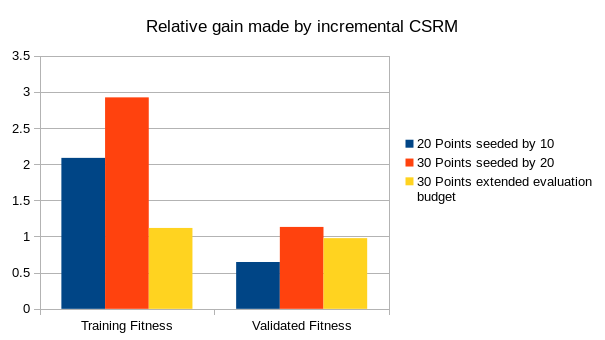
\includegraphics[width=\textwidth,height=\textheight,keepaspectratio]{figures/incrementalgain.png}
    \caption{Incremental fitness gain in CSRM.}
    \label{fig:incrementalgain}
\end{figure}
\subsubsection{Convergence behavior}
\paragraph{Fitness distribution}
In Figures \ref{fig:incrementalseededconvergence}\ref{fig:incrementalconvergence}\ref{fig:incrementaldoubleconvergence} we see how the convergence process evolves over time. If we compare the fitness plot we clearly see that the seeded process has a different distribution compared with the unseeded runs. Around generation 1000 the convergence rate slows. Doubling the phases has little effect on the fitness distribution. 
% TODO check plots of fitness, make sure they correspond to those runs
\paragraph{Operator effectiveness}
In the plots we see operator success rate and operator gains visualized. The first is the ratio between applications of an operator that leads to improvement in fitness versus the total number of applications. The trendline is obtained by a cubic fit.This gives us an indication whether an operator is still effective, in particular it gives us the fraction of the population that is improved each generation by the operator. The second plot is the mean gain of an operator, it reflects how much the fitness of each generation is improved by an operator. The distinction is important, if fitness is improved by very small amounts the success rate will be high but the gain low. These statistics offer an insight into the convergence characteristics over generations. Instead of relying only on the end result we can directly observe the effects of the operators. For our comparison we see that there is little difference in gain or success rate between the three runs.
\paragraph{Constant folding}
The percentage of nodes saved is similar for all three runs. The plots show that constant subtrees are introduced at a constant rate and folded at the end of each generation. The savings plotted also give an indication of the potential increase in nodes that could take place if folding was not implemented. 
 \begin{figure}
    \begin{subfigure}{0.5\textwidth}
        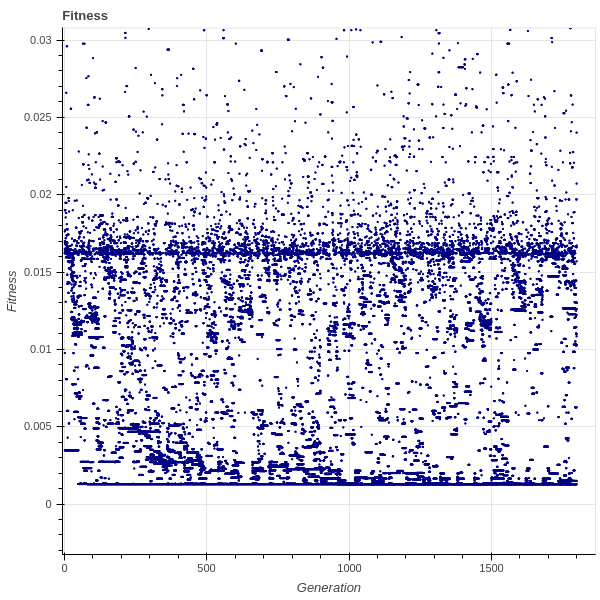
\includegraphics[width=0.8\linewidth]{figures/incrementalfitness30s.png}
        \caption{Fitness.}
    \end{subfigure}
    \begin{subfigure}{0.5\textwidth}
        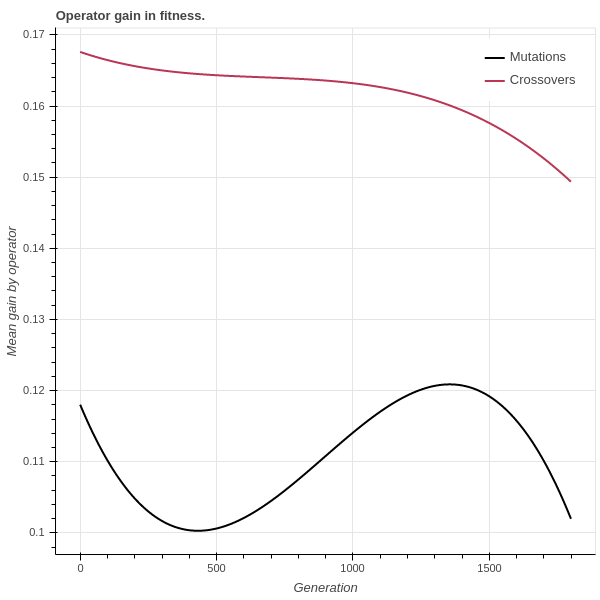
\includegraphics[width=0.8\linewidth]{figures/incrementaloperatorgain30s.png}
        \caption{Operator gain.}
    \end{subfigure}
        \begin{subfigure}{0.5\textwidth}
        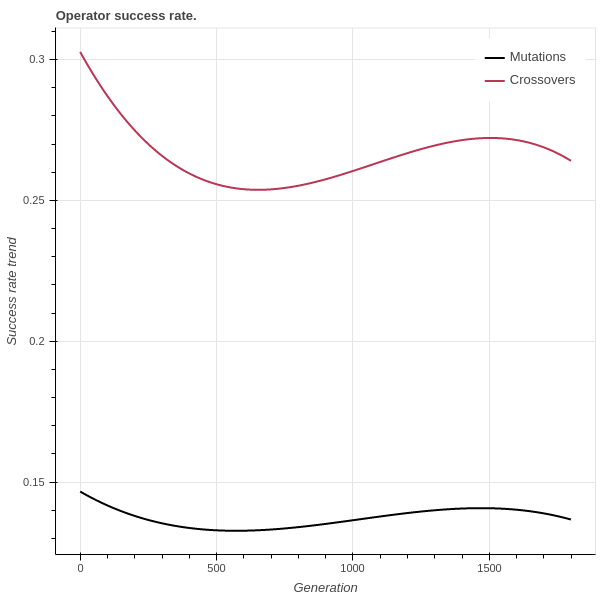
\includegraphics[width=0.8\linewidth]{figures/incrementaloperatorsuccessrate30s.png}
        \caption{Operator success rate.}
    \end{subfigure}
    \begin{subfigure}{0.5\textwidth}
        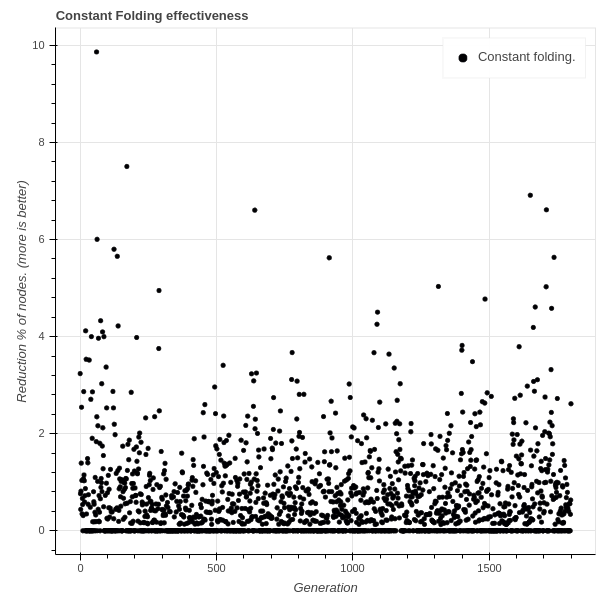
\includegraphics[width=0.8\linewidth]{figures/incrementalconstfolding30s.png}
        \caption{Constant folding savings.}
    \end{subfigure}
    \caption{Convergence behavior of incremental symbolic regression with 10-20-30 split.}
    \label{fig:incrementalseededconvergence}
\end{figure}
 \begin{figure}
    \begin{subfigure}{0.5\textwidth}
        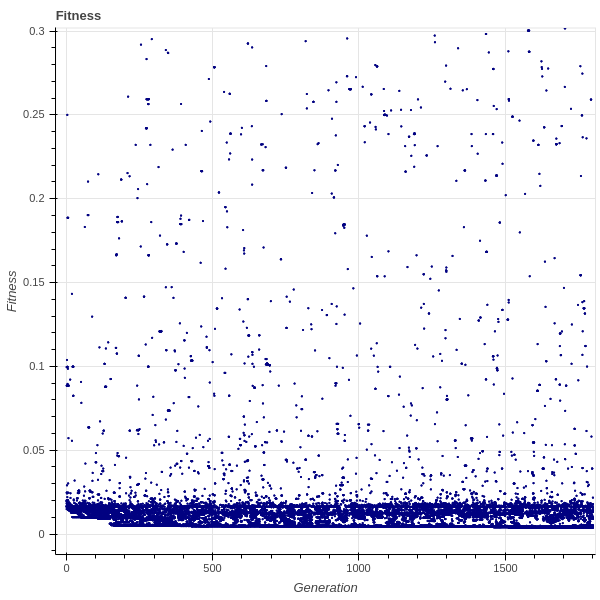
\includegraphics[width=0.8\linewidth]{figures/incrementalfitness30.png}
        \caption{Fitness.}
    \end{subfigure}
    \begin{subfigure}{0.5\textwidth}
        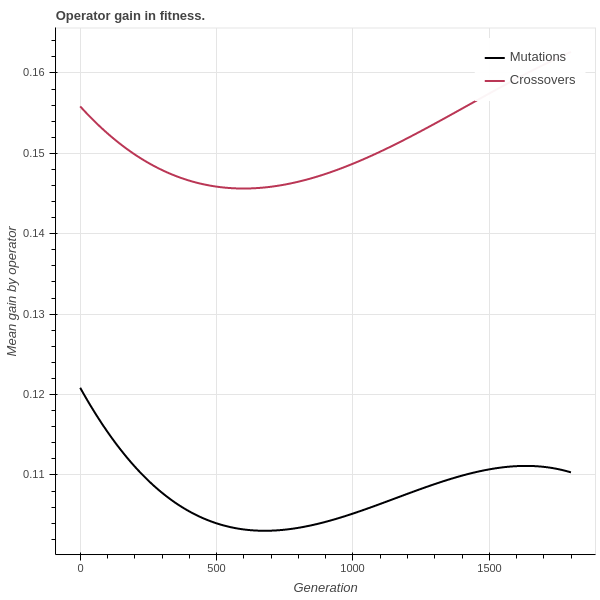
\includegraphics[width=0.8\linewidth]{figures/incrementaloperatorgain30.png}
        \caption{Operator gain.}
    \end{subfigure}
        \begin{subfigure}{0.5\textwidth}
        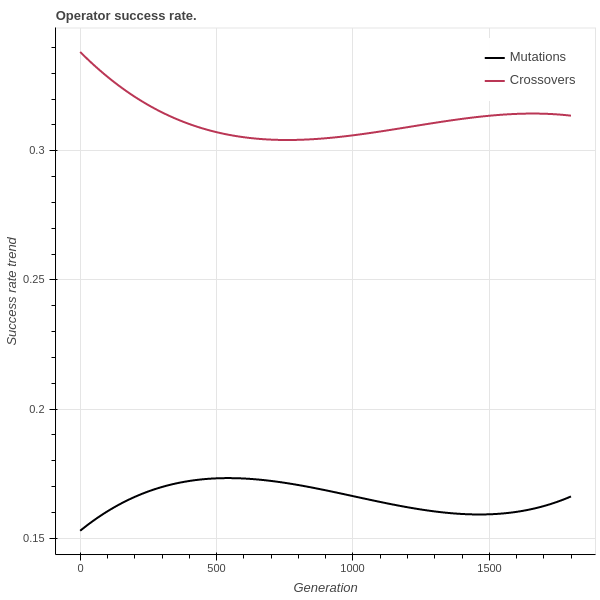
\includegraphics[width=0.8\linewidth]{figures/incrementaloperatorsuccessrate30.png}
        \caption{Operator success rate.}
    \end{subfigure}
    \begin{subfigure}{0.5\textwidth}
        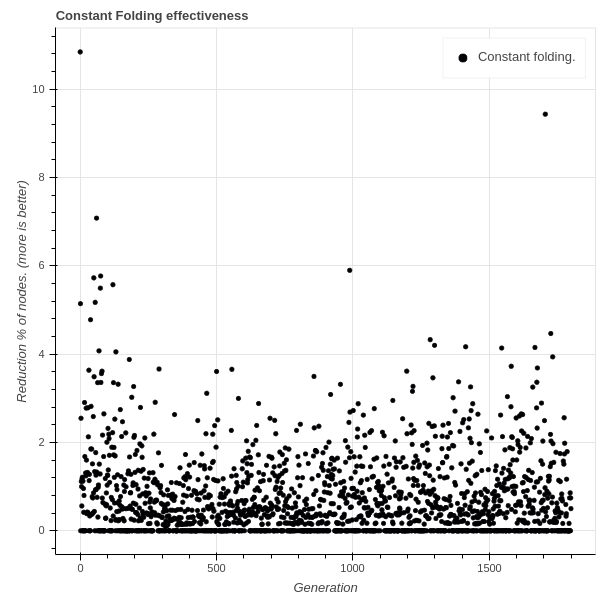
\includegraphics[width=0.8\linewidth]{figures/incrementalconstfolding30.png}
        \caption{Constant folding savings.}
    \end{subfigure}
    \caption{Convergence behavior of incremental symbolic regression without split.}
    \label{fig:incrementalconvergence}
\end{figure}
% [bcardoen@localhost src]$ python3 -m gp.paralleldriver -c 1 -t none -g 60 -p 20 -f 60 -x doe/input.csv -y doe/output.csv -m 6 -v -d 30 -q 3 -i 3

 \begin{figure}
    \begin{subfigure}{0.5\textwidth}
        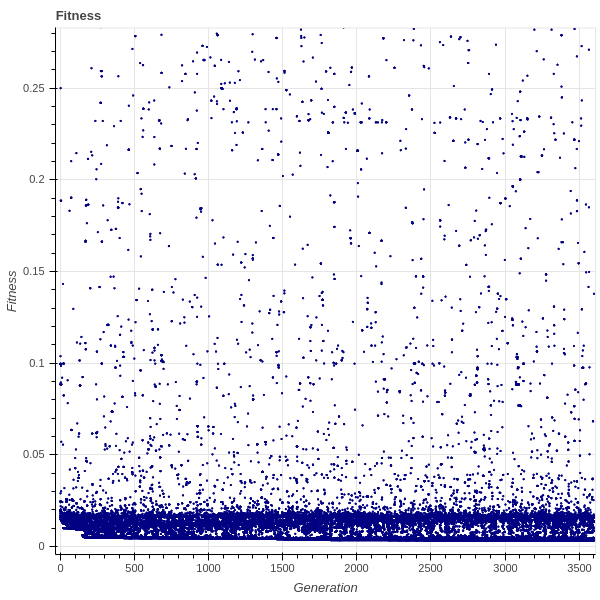
\includegraphics[width=0.8\linewidth]{figures/incrementalfitness30d.png}
        \caption{Fitness.}
    \end{subfigure}
    \begin{subfigure}{0.5\textwidth}
        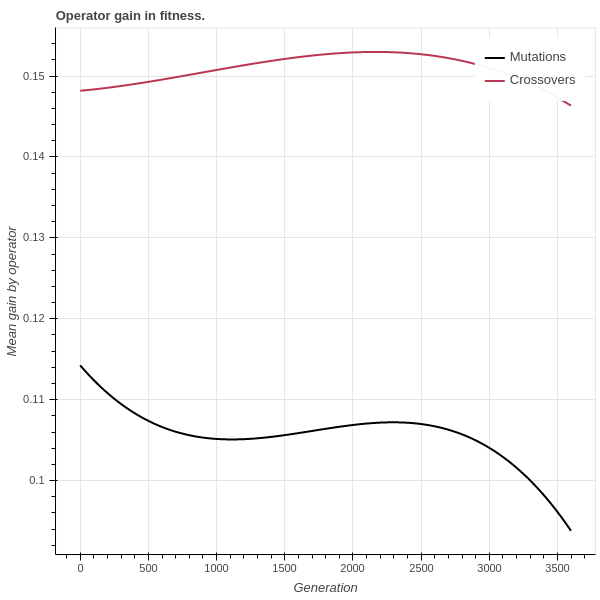
\includegraphics[width=0.8\linewidth]{figures/incrementaloperatorgain30d.png}
        \caption{Operator gain.}
    \end{subfigure}
        \begin{subfigure}{0.5\textwidth}
        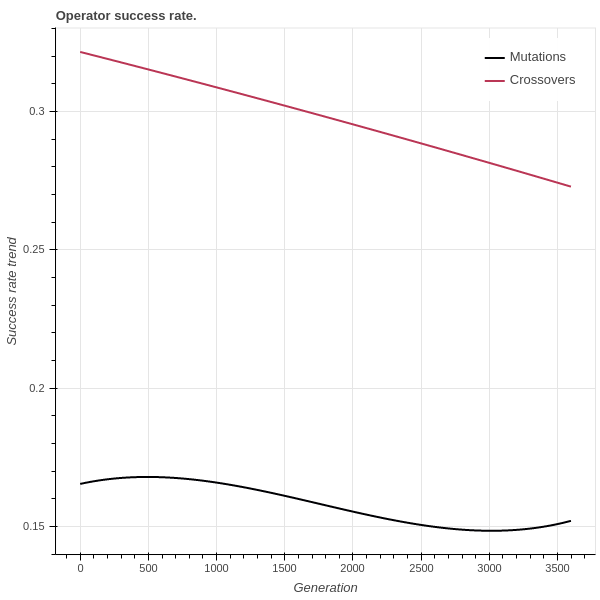
\includegraphics[width=0.8\linewidth]{figures/incrementaloperatorsuccessrate30d.png}
        \caption{Operator success rate.}
    \end{subfigure}
    \begin{subfigure}{0.5\textwidth}
        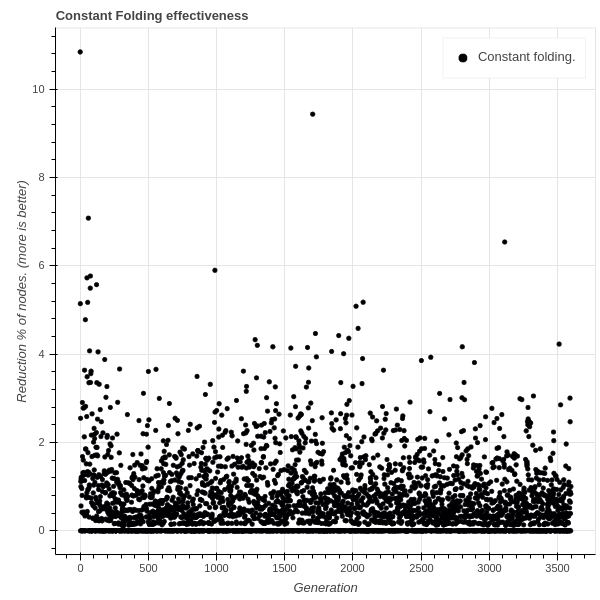
\includegraphics[width=0.8\linewidth]{figures/incrementalconstfolding30d.png}
        \caption{Constant folding savings.}
    \end{subfigure}
    \caption{Convergence behavior of incremental symbolic regression with identical computational cost as 10-20-30 split.}
    \label{fig:incrementaldoubleconvergence}
\end{figure}
\subsection{Conclusion}
We have seen that incremental use of symbolic regression can, when applied judiciously, increase convergence compared to a blind search with the same computational cost. In addition to obtaining improved results we can integrate it with a simulator that produces output in parallel.
